\section{Case Study: Maximum Subarray}

\subsection*{Steps}

\begin{enumerate}
	\item Divide the array in half into two subarrays (left subarray and right subarray).
	\item Recursively repeat this process until each subarray consists of only one element. At this point, the maximum sum of each subarray is the single element.
	\item Calculate the maximum sum for the cross section.
	\begin{enumerate}
		\item Start from the mid-point of the subarray.
		\item Sum up all numbers from the mid-point to the first element. Whenever the sum exceeds its previous value, that value becomes the left sum.
		\item Sum up all numbers from the mid-point+1 to the last element. Whenever the sum exceeds its previous value, that values becomes the right sum.
		\item The summation of the left sum and the right sum becomes the maximum sum for the cross section. Note: If all the elements in the subarrays are negative, then the left and right sum will return 0 by default.
	\end{enumerate}
	\item Compare the maximum sum from the left array, right array, and cross section. The largest of the three get returned.
\end{enumerate}

\subsection*{Recurrence Relation}
$$
T(n) = 2T(\frac{n}{2}) + \Theta(n)
$$

\subsection*{Complexity}
$$
T(n) \in \Theta(n \cdot lg(n))
$$

\newpage

\subsection{Example}
\textbf{Find the maximum subarray of the following array: $\{-2, 1, -3, 4, -1, 2, 1, -5, 4 \} $ }

\subsubsection*{Divide}
\begin{figure}[h]
	\centering
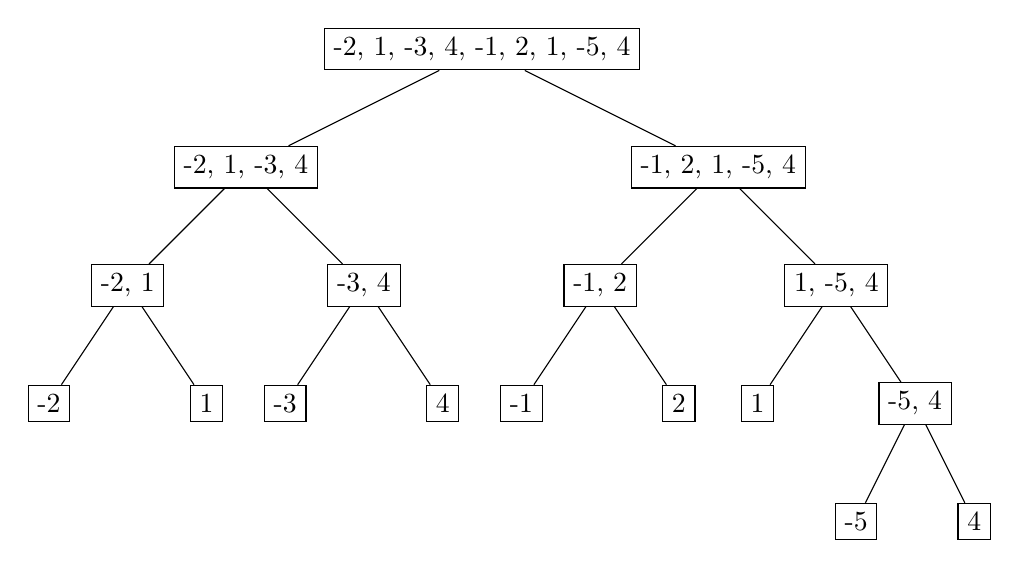
\begin{tikzpicture}[level/.style={sibling distance=60mm/#1}]
	\node [rectangle,draw] {-2, 1, -3, 4, -1, 2, 1, -5, 4}
		child {
			node [rectangle,draw] (a) {-2, 1, -3, 4}
				child {
					node [rectangle,draw] {-2, 1}
						child {
							node [rectangle, draw] {-2}
						}
						child {
							node [rectangle, draw] {1}
						}
				}
				child {
					node [rectangle,draw]{-3, 4}
					child {
						node [rectangle, draw] {-3}
					}
					child {
						node [rectangle, draw] {4}
					}
				}
		}
		child {
			node [rectangle,draw] (b) {-1, 2, 1, -5, 4}
				child {
					node [rectangle,draw]  {-1, 2}
						child {
							node [rectangle, draw] {-1}
						}
						child {
							node [rectangle, draw] {2}
						}
				}
				child {
					node [rectangle,draw]  {1, -5, 4}
						child {
							node [rectangle, draw]  {1}
						}
						child {
							node [rectangle, draw] {-5, 4}
								child {
									node [rectangle, draw] {-5}
								}
								child {
									node [rectangle, draw] {4}
								}
						}
				}
		};
\end{tikzpicture}
\end{figure}

\subsubsection*{Combine}
\begin{table}[h]
	\centering
	\begin{tabular}{| >{$}c<{$} | >{$}c<{$} |  >{$}c<{$} | >{$}c<{$} | >{$}c<{$} | >{$}c<{$} | >{$}c<{$} |}
		\hline
		\text{Depth}
			&	\text{Left Subarray}
			&	\text{Right Subarray}	
			&	\text{Max(Left)}	
			&	\text{Max(Right)}	
			&	\text{Max(Cross)}
			&	\text{Return}\\
		\hline
		4		
			&	\{ -5 \}	
			&	\{ 4 \}
			& 	-5
			&	4
			&	4
			&	4\\
		\hline
		3
			&	\{ -2 \}
			&	\{ 1 \}
			&	-2
			&	1
			&	1
			&	1\\
		\hline
			&	\{ -3 \}
			&	\{ 4 \}
			&	-3
			&	4
			&	4
			&	4\\
		\hline
			&	\{ -1 \}
			&	\{ 2 \}
			&	-1
			&	2
			&	2
			&	2\\
		\hline
			&	\{ 1 \}
			&	\{ -5, 4 \}
			& 	1
			&	4
			&	4
			&	4\\
		\hline
		2
			&	\{ -2, 1\}
			&	\{ -3, 4\}
			&	1
			&	4
			&	1
			&	4\\
		\hline
			&	\{ -1, 2 \}
			&	\{ 1, -5, 4 \}
			&	2
			&	4
			&	3
			&	4\\
		\hline
		1
			&	\{ -2, 1, -3, 4 \}
			&	\{ -1, 2, 1, -5, 4 \}
			&	4
			&	4
			&	6
			&	6\\
		\hline
	\end{tabular}
\end{table}
$$
\text{The maximum sum is 6 from indices 3 to 6.}
$$

\subsubsection*{Visualization of Finding the Max of Cross Section}
Taking depth = 1 with left subarray = $\{ -2, 1, -3, 4 \}$ and right subarray = $\{ -1, 2, 1, -5, 4 \}$.

\begin{minipage}[t]{0.5\linewidth}
	$$
	\text{Cross Section Left Sum}
	$$
	$$
	\{ -2, 1, -3, 4, \underbrace{-1}_{\text{Mid}}, 2, 1, -5, 4 \}
	$$
	$$
	\{ -2, 1, -3, 4, \underbrace{-1}_{\text{-1}}, 2, 1, -5, 4 \}
	$$
	$$
	\{ -2, 1, -3, \underbrace{4, -1}_{\text{3}}, 2, 1, -5, 4 \}
	$$
	$$
	\{ -2, 1, \underbrace{-3, 4, -1}_{\text{0}}, 2, 1, -5, 4 \}
	$$
	$$
	\{ -2, \underbrace{1, -3, 4, -1}_{\text{1}}, 2, 1, -5, 4 \}
	$$
	$$
	\{ \underbrace{-2, 1, -3, 4, -1}_{\text{-1}}, 2, 1, -5, 4 \}
	$$
	$$\text{Max Left Sum} = 3$$
\end{minipage}
\begin{minipage}[t]{0.5\linewidth}
	$$
		\text{Cross Section Right Sum}
	$$
	$$
	\{ -2, 1, -3, 4, -1, \underbrace{2}_{\text{Mid + 1}}, 1, -5, 5 \}
	$$
	$$
	\{ -2, 1, -3, 4, -1, \underbrace{2}_{\text{2}}, 1, -5, 5 \}
	$$
	$$
	\{ -2, 1, -3, 4, -1, \underbrace{2, 1}_{\text{3}}, -5, 5 \}
	$$
	$$
	\{ -2, 1, -3, 4, -1, \underbrace{2, 1, -5}_{\text{-2}}, 4 \}
	$$
	$$
	\{ -2, 1, -3, 4, -1, \underbrace{2, 1, -5, 4}_{\text{2}} \}
	$$
	$$
	\text{Max Right Sum} = 3
	$$
\end{minipage}


